\documentclass[10pt,a4paper]{article}
\usepackage[utf8]{inputenc}
\usepackage[spanish,mexico]{babel} 
\usepackage{amsfonts}
\usepackage{amsmath}
\usepackage{amssymb}
\usepackage{multicol}
\usepackage{graphicx}
\usepackage{subcaption}
\usepackage{float}
\usepackage{lipsum}
\usepackage{xcolor}
\usepackage[rightcaption]{sidecap}
\usepackage{array}
\usepackage{framed}
\usepackage{wrapfig}
\definecolor{shadecolor}{RGB}{224,238,238}
\usepackage{listings}
\usepackage[hidelinks]{hyperref}
\usepackage{pdfpages}
\usepackage{pdflscape}
\usepackage{verbatim}
\pagestyle{plain}
\usepackage[nottoc]{tocbibind}
\usepackage{times}

\graphicspath{{../04_Images/}}

% Márgenes
\usepackage[top=2.5cm, bottom=2.5cm, left=3.0cm, right=2.5cm]{geometry}

\title{Desarrollo de un Modelo de Aprendizaje Incremental de Redes Neuronales Artificiales Aplicado al Conjunto de
Datos Optdigit}

\makeindex

\begin{document}

    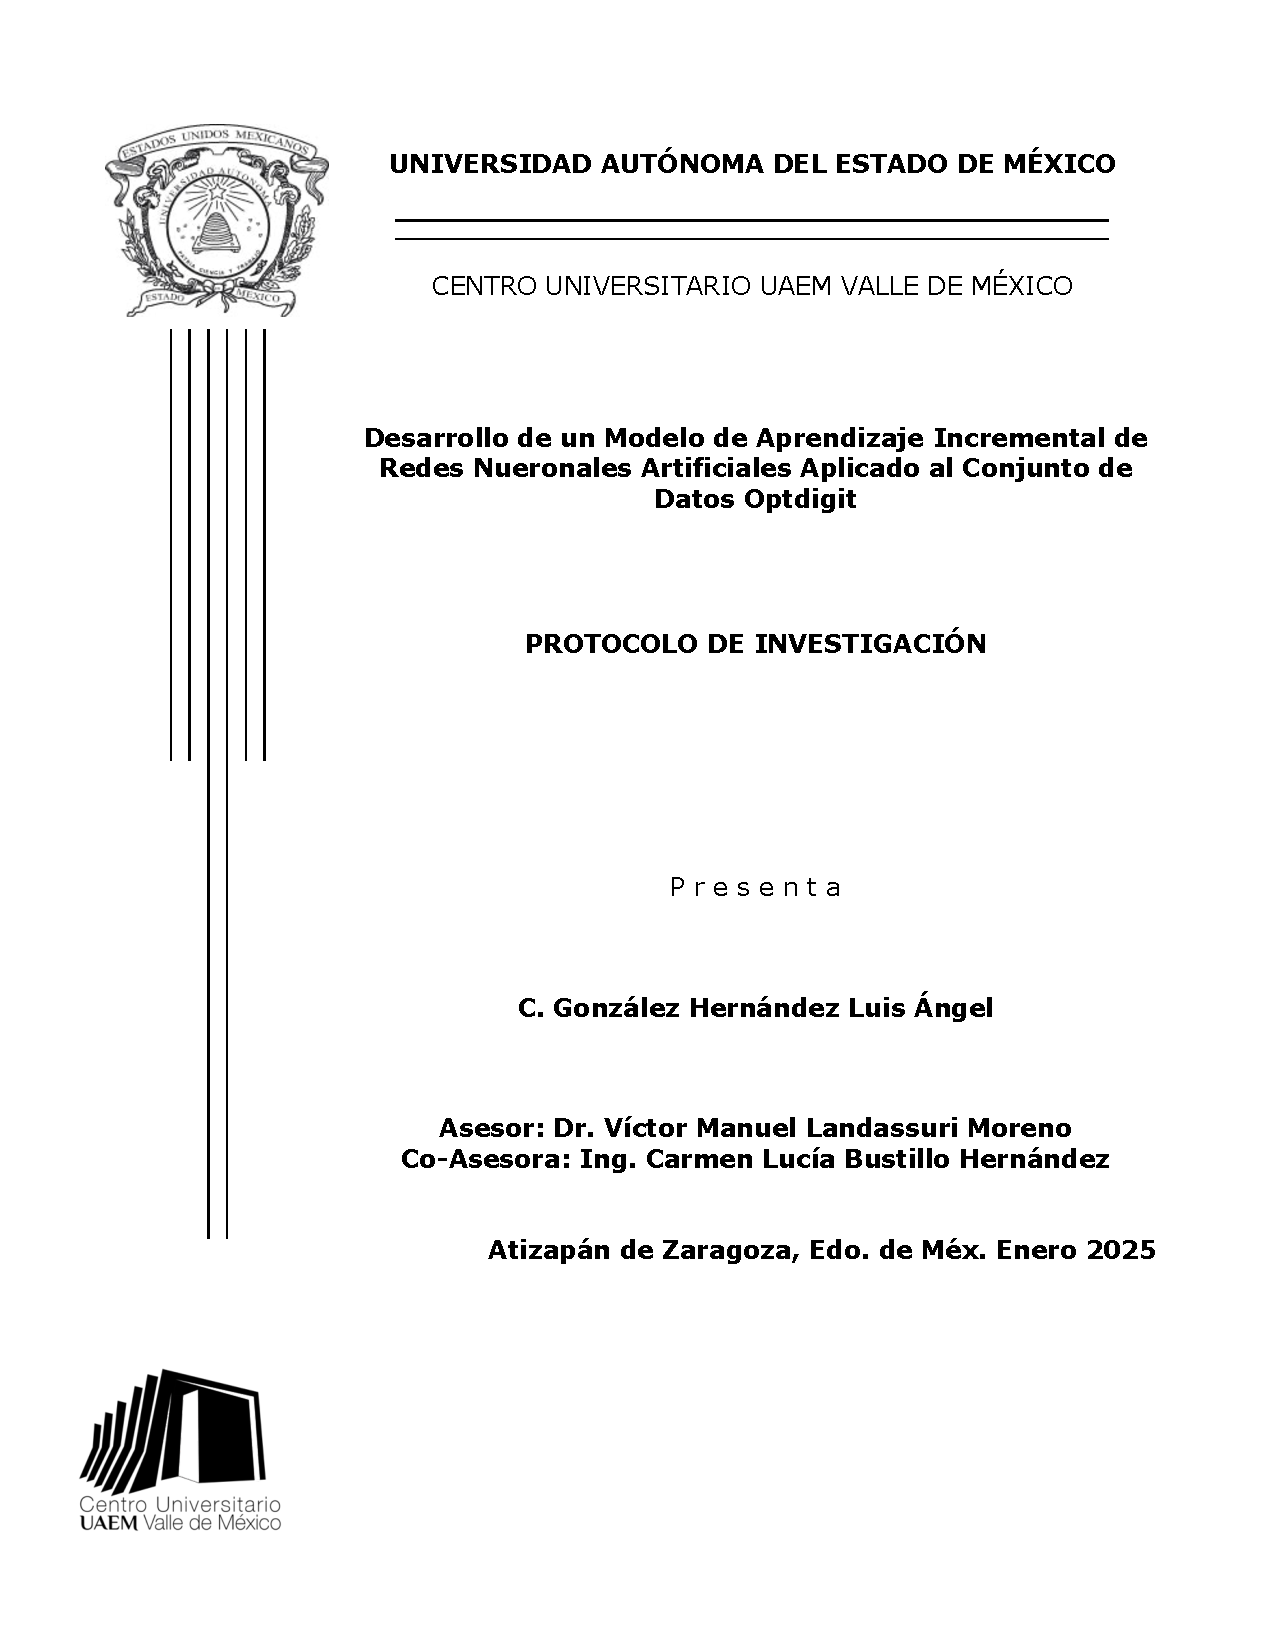
\includepdf{../02_Chapters/portada}
    \tableofcontents
    \listoffigures
    \maketitle
    \begin{abstract}
        En un enfoque normal, primero se entrena el modelo con un conjunto de datos inicial, y una vez que el modelo está listo, se utiliza para realizar predicciones. Sin embargo, si llega nueva información, es necesario reentrenar el modelo desde cero, utilizando tanto la información histórica como la nueva. Este proceso puede ser computacionalmente costoso y poco eficiente, especialmente cuando se manejan grandes volúmenes de datos.
        
        El aprendizaje incremental es un área de la Inteligencia Artificial que permite agregar nuevo conocimiento a un modelo (e.g., Redes Neuronales Artificiales) sin la necesidad de entrenar el modelo con toda la información histórica de la tarea en cuestión \cite{bullinaria2009}. En el presente trabajo de investigación se utilizará el modelo de Redes Neuronales Artificiales enfocado en la clasificación de dígitos escritos a mano, empleando el algoritmo de entrenamiento de backpropagation, con redes Multicapa Perceptron y duplicación de pesos múltiples, simulando memoria a corto y largo plazo para mejorar los resultados presentados en \cite{bullinaria2009}.
        \end{abstract}
        
        \textbf{Palabras clave:} Aprendizaje incremental, Redes Neuronales Artificiales, Clasificación de dígitos.

    \section{Introduccion}

El aprendizaje incremental es un método el cual a sido implementado en el área de la inteligencia artificial, ya que al realizar tareas especificas de dicha rama nos 
ayuda a optimizarla para que el algoritmo sea más eficiente.
Cualquier tipo de aprendizaje puede ser considerado aprendizaje incremental si el problema a resolver tiene un entrenamiento simple, adem\'as este tipo de algoritmo es conocido como \textit{algoritmo lineal sin memoria},
en la mayor\'ia de los casos este tipo de aprendizaje es el preferido o favorito por los desarrolladores \cite{GiraudCarrier2000}.

Las redes neuronales artificiales (RNAs) son procesos matem\'aticos los cuales son utilizados en el \'area de Machine Learning para 
la resoluci\'on de problemas no lineales, estos deben de pasar por una funci\'on de activaci\'on la cual es una multiplicaci\'on 
entre lo valores otrogados, al ser procesados por las capas que contenga la neurona, obtendremos un valor distinto al de entrada.

Adem\'as son una distribuci\'on muy conocida de parte del Machine Learning, de otra manera es el poder que tienen las computadoras para una buena estructura distribuida en paralelo y una buena habilidad de aprendizaje, 
este modelo computacional se define por medio de las neuronas biologicas las que son encargadas de que el ser humano pueda aprender o distinguir de distintos aspectos, este tipo de 
metodo es motivado para poder obtener la meta de un buen aprendizaje de maquina \cite{liu2015}.

Un factor importante para esta rama es la perdida de memoria, este es un problema biol\'ogico, el cual tanto afecta a los humanos como a las maquinas, es por eso que se han elaborado distintos
experimentos para poder convatir esta problematica.
Uno de  estos es el caso de John Bullinaria, quien maneja la arquitectura de doble peso, ya que en su experimento da a notar que mejora la utilizaci\'on del aprendizaje incremental, esto se logro 
con sistemas existentes como lo es Learn++.

Cabe mencionar que el experimento realizado fue un problema de generalizaci\'on m\'as comunes, pero se necesitan m\'as evidencias 
de que usando esta metodolog\'ia sirve para utilizarlo no solamente en tareas generalizadas, adem\'as se espera un mejor rendimiento \cite{Bullinaria2009}.  \\


\section{Planeamiento}

    Indicar de forma general como es el funcionamiento de las redes neuronales en el uso general, como es que se produce la falta de memoria en 
    estos modelos de predicciones. Poner en pr\'actica los modelos de experimentación de John Bullinaria para comprobarlos con
    problematicas m\'as robustas y optimizarlo para que sea un m\'etodo eficiente.
    \section{Planeamiento}

    Las Redes Neuronales Artificiales tienen la habilidad de poderse aprender una tarea, 
    y poder hacer o resolver tareas de predicción o clasificación básicamente. En este 
    sentido, con algoritmos de aprendizaje como el Backpropagation, permite ajustar los 
    pesos de una RNA para que esta pueda empezar a resolver una tarea particular.  No 
    obstante, muchas de las tareas que se resuelven en la vida diaria, van generando mas 
    información con el tiempo, por ejemplo, el comportamiento de un una serie financiera, 
    o bien la predicción del clima en una determinada región. Así,  se tiene el aprendizaje 
    incremental, siendo un método poco explorado,  enfocado en poder aprender nueva información del 
    problema, sin tener que volver a entrenar todo el modelo con la información anterior, y la 
    nueva que acaba de llegar, esto es, en los modelos actuales de aprendizaje máquina, si se usa 
    un conjunto de datos para entrenar un modelo en especifico, dicho modelo es funcional para 
    dicho conjunto de datos y la información que ello representa. Sin embargo, si es necesario 
    incorporar nueva información al modelo, es necesario recolectar dicha información nueva, 
    agregarla a la que se tenia anteriormente, y volver a entrenar todo el modelo para que \'este 
    pueda incorporar la nueva información.

    De esta forma, una red ya entrenada con un primer conjunto de datos $d_{1}$ se desea entrenar 
    con un nuevo conjunto de datos del mismo problema $d_{2}$, al entrenar la red con $d_{2}$ se 
    perderá en conocimiento aprendido por $d_{1}$.  Si no se desea utilizar un modelo de aprendizaje 
    incremental, se tendría que juntar el conjunto $d_{1}$ y $d_{2}$ en un solo conjunto y volver a 
    entrenar la RAN para así poder incorporar el nuevo conocimiento ($d_{2}$) a la RNA. Si se desea 
    utilizar el método de aprendizaje incremental, se puede entrenar en un primer moemnto a la red 
    con el conjunto $d_{1}$, posteriormente con $d_{2}$ teniendo poca perdida de información de $d_{1}$. 
    Si más adelante llega mas información del problema ($d_{3}$) que se desee incorporar a la base 
    de conocimientos de la RNA, entonces solo habrá que entrenar la RNA con $d_{3}$ usando el modelo 
    incremental para tener una p\'erdida mínima de información de $d_{1}$ y $d_{2}$. 

    De esta forma, el presente trabajo tomar\'a como base la investigación de \cite{bullinaria2009}, 
    en donde utiliza una configuración de pesos dobles (a una RNA se duplican todos sus pesos), 
    donde a una capa de pesos duplicados se enlaza con una tasa de aprendizaje alta, para simular un 
    rápido aprendizaje, y por ende simular lo que sería memoria a corto plazo. En su contraparte, 
    la segunda capa de pesos duplicados, se enlaza con una tasa de aprendizaje baja para aprender 
    lentamente un problema, simulando la memoria a largo plazo.  Es decir, al momento de aprender una 
    tarea nueva,  una capa de pesos aprenderá muy rápido la nueva tarea (tasa alta de aprendizaje) y 
    por ende olvidará más rápidamente los datos ya aprendidos anteriormente, por otro lado, la segunda 
    capa de pesos duplicados, aprenderá muy lentamente los nuevos datos que llegan, y por ende olvidando 
    poco la información que anteriormente se aprendió.  Considerando ello y también que la 
    RNA trabaja en conjunto con ambas capas de pesos duplicados, se pondera la salida de la RNA para 
    que pueda contemplar la información nueva que se acaba de agregar a la RNA, en ambas capas, así como 
    la información que se acaba de olvidar de ambas capas de pesos.

    El problema principal del aprendizaje incremental mostrado en \cite{bullinaria2009}, es que entre 
    más conjuntos de datos nuevos que lleguen, mas se olvidaran los primeros conjuntos que se aprendieron, 
    lo cual no es tan útil si se contempla que en el futuro de una RNA podrán existir 10 o 20 etapas de 
    entrenamiento incremental con nuevos conjuntos de datos que se vayan recolectando.

    Por ello es indispensable poder explorar nuevas configuraciones de RNAs que permitan mejorar los 
    métodos actuales para permitir una menor cantidad de olvido conforme llegue nueva información al 
    modelo. Donde al igual que en trabajos anteriores,  el presente trabajo se basará en conceptos de 
    memoria a corto y largo plazo, y en lugar de hacer una copia de los pesos actuales y tener dos 
    tasas de aprendizaje, una rápida para simular la memoria a corto plazo, y otra tasa de aprendizaje 
    para simular la memoria a largo plazo, se explorará por hacer mas copias de los pesos, teniendo más 
    tasas de aprendizaje que operen en cada una de dichas copias.
    
    \chapter{Objetivos}
    Diseñar una red neuronal artificial para aprendizaje incremental basada en el principio de la memoria a corto y largo plazo, buscando usar más de dos capas de pesos duplicados para el reconocimiento de dígitos, y con una menor p\'erdida de información de trabajos previos.
    \section{Objetivos Específicos}
        \begin{enumerate}
            \item Implementar el algoritmo mostrado en \cite{bullinaria2009} para el reconocimiento de dígitos con aprendizaje a corto y largo plazo con los parámetros que ahí se indican.
            \item Obtener el conjunto de datos de Optical Digits, limpiar los datos y prepararlos según lo indicado con \cite{bullinaria2009}.
            \item Separar el conjunto de entrenamiento y de prueba de acuerdo a lo que se explica en el artículo de Bullinaria y probar el primer código implementado en miras de comprobar los resultados previamente mostrados en \cite{bullinaria2009}.
            \item Tomar como base el algoritmo implementado, y extenderlo para permitir mas de dos pesos duplicados, aplicando el conjunto de datos previamente mostrado.
            \item Comparar ambas implementaciones en busca de una reducción significativa de las tasas de aprendizaje con respecto a trabajos previos en la literatura.
        \end{enumerate}
    \section{Hipótesis}
    Al tener m\'as de dos capas de pesos duplicados con sus respectivas tasas de aprendizaje, permite tener un menor olvido de la información previa aprendida, en un modelo de aprendizaje incremental con redes neuronales artificiales del tipo MLP, al usar el algoritmo de Backpropagation.  
%(AQUÍ DE FAVOR SÓLO REVISA QUE EL ACRÓNIMO MLP - MULTI CAPA PERCEPTRON DEL INGLES MULTILAYER PERCEPTRON - SE HAYA DESCRITO ANTERIORMENTE)
    \chapter{Justificación}
	
	
    Las redes neuronales permiten el aprendizaje automático y la resolución 
    de distintos problemas,  pero como se comentó anteriormente,  las técnicas 
    de aprendizaje máquina, tienen una deficiencia que es al momento de aumentar 
    los nuevos bloques de datos que llegan para aprender,  se obtiene un deterioro 
    en el rendimiento de aprendizaje de información y olvido de la información anterior \cite{bullinaria2009}.\\
    
    Los resultados que se han obtenido no han funcionado a la perfección, la 
    memoria a corto plazo olvida poco pero va olvidando, y lo ideal sería que no 
    olvidara. Biológicamente, los humanos pueden aprender nuevas tareas, o información 
    nueva de un problema, y no olvida de forma significativa lo que anteriormente 
    aprendió, no obstante, eso no pasa actualmente con las RNA y en general con 
    cualquier algoritmo de aprendizaje máquina. En otro sentido, los humanos 
    ya tienen cierta configuración en el cerebro que les permite aprender como 
    se hace actualmente,  y se puede afirmar que por el momento no hay ningún 
    procedimiento (ya sea quirúrgico o no) que permita modificar la estructura del cerebro 
    para aprender mas y olvidar menos.\\

    No obstante,  computacionalmente nada puede impedir que se experimente con más 
    configuraciones y llegar al punto en donde toda la información que ingrese a un 
    modelo (por ejemplo RNAs) se acumule, y si no hay problema de almacenamiento, que \'esta se siga 
    acumulando y que no olvide, esto podría ser bueno en diversas situaciones.\\

    Desde un punto de vista computacional, si llega nueva información y no se ocupa aprendizaje 
    incremental, esto implicar\'a volver a entrenar todo el sistema con la información anterior y 
    la actual (por ejemplo, $d_{1}$ y $d_{2}$) y considerando que una de las desventajas que tienen la 
    RNAs es que el entrenamiento es un cuello de botella, siendo este donde se lleva la mayor 
    parte de cómputo y por consiguiente de energía. Lo mencionado anteriormente implica que volver a entrenar con toda 
    la información acumulada, gastará más energía y tiempo, que si solo se entrena con la nueva 
    información que llega al modelo. En su contraparte,  existe una gran variedad de herramientas,
    las cuales permiten codificar una red neuronal artificial con librerías ya preexistentes, para esta investigación solo se 
    expondrán 2 empresas, siendo estas las más importantes: Microsoft y Google. 
    La primera cuenta con la plataforma de Azure que renta una maquina virtual donde se puede 
    programar en Python, y la segunda, cuenta con Google Colab que de igual forma brinda 
    una m\'aquina virtual para realizar experimentos de Maching Learning, la \'unica diferencia 
    contra Azure es que dicha herramienta es gratuita, y una similitud que tienen es que en ambas herramientas
    se puede programar en el mismo lenguaje.\\

    Como se puede observar, las herramientas mencionadas permiten la programación en Pyhton, y esto se debe a que 
    dicho lenguaje es una herramienta de software libre que no requiere licencia, es relativamente 
    fácil poder depurar un código y permite acelerar más el desarrollo de aplicaciones,  a diferencia 
    de otros lenguajes más estructurados como C o Java, adem\'as tiene m\'as librerías para el 
    desarrollo de Maching Learning, por ejemplo, TensorFlow, Numpi, entre otras. \\

    TensorFlow es una librería de Python que permite construir y entrenar redes neuronales para 
    detectar patrones y razonamientos usados por los humanos, en la presente investigaci\'on se 
    usar\'a dado a que favorece la creaci\'on de una RNA, permite la elaboraci\'on de cualquier 
    tipo de algoritmo de Machine Learning, cabe mencionar que también se puede usar para Deep Learning, 
    facilita la adquisici\'on de datos modelos de capacitaci\'on, predicciones y refinamiento de 
    resultados, est\'a disponible para el uso en computadores personales, pero es recomendado 
    usarlo en su propio editor en la nube que es Colab.\\
    
    Keras es un framework de alto nivel para 
    el aprendizaje, escrito en Python y capaz de correr sobre los frameworks TensorFlow, por esta razón se usar\'a para la presente investigación, pues facilita los procesos de experimentación rápida, y ya que al ejecutarse en TensorFlow, por consiguiente se puede ejecutar en Colab.
    \section{Delimitación}
\label{sec:delimitation}
	
	
    En la presente investigación solamente se utilizará redes neuronales del tipo perceptr\'on multicapa,  donde 
    cabe mencionar que este no es el único tipo de red que existe, i.e., también se tiene Redes Neuronales Convolucionales (RNC), Redes Neuronales Recurrentes (RNR) o bien Redes de Base Radial (RBR) \cite{royo2021}. Así mismo, no se abordará el uso de técnicas d eoptimiación como lo son los algoritmos genéticos, y unicamente se limitará a explorar la mejora en rendimiento al tener más de dos capas duplocadas de pesos en la red con aprendizaje incremental.  Así mismo, no se abordarán modelos como las redes profundas u otro conjunto de datos y se limitará el trabajo a lo antes mencionado.



    \section{Consecuencias}

    Si el experimento funciona a la perfecci\'on ocurrir\'a lo siguiente:
    \begin{enumerate}
        \item Habrá menos olvido.
        \item El aprendizaje tomará menos tiempo.
    \end{enumerate}

    Como se menciona antes, se van a poder ingresar m\'as datos sin 
    tener que volver a codificar el modelo.\\
    Los modelos de predicci\'on van a ser m\'as precisos, porque se podrán ingresar 
    datos mensualmente o hasta semanalmente, esto provocar\'a que el proyecto est\'e trabajando 
    con datos actuales.

    Pueden funcionar para proyectos y predicciones tan simples, por ejemplo, la preiddci\'on climatol\'ogica, 
    predicciones de la bolsa de valores, predicci\'on del Bitcoin, entre otras.

    \section{Marco Teórico}

    \subsection{Redes Neuronales Artificiales}

        Las redes neuronales artificiales (RNA) son modelos computacionales dentro de la Inteligencia Artificial que contienen unidades de procesamiento simples llamadas neuronas. Estas se inspiran en el cerebro humano, basándose en la conectividad entre neuronas y el aprendizaje que pueden tener. Un perceptrón o neurona (artificial) solo resuelve problemas lineales y tiene la siguiente forma:

        \begin{figure}[H]
            \centering
            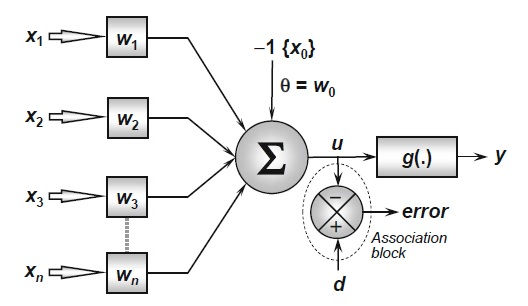
\includegraphics[width=\columnwidth]{ANN.jpg}
            \caption{Red Neuronal Artificial Básica}
            \label{fig:nerural_network}
        \end{figure}

        Donde $\Sigma$ es la representación matemática de la neurona. $x_1$, $x_2$, \dots ,$x_n$ son las variables de entrada a la red, y $w_1$, $w_2$, \dots ,$w_n$ son los pesos con los cuales se ponderan las entradas, es decir, se multiplican cuando la información entra en la neurona. Posteriormente, se suman todos esos valores: $w_1 x_1 + w_2 x_2 + w_3 x_3$. 

        Al revisar la fórmula anterioir, se puede observar que se parece a la operación de una regresión, la cual es: $y = w_0 + w_i x_i$. De esta manera, internamente la neurona realiza una regresión lineal. El parámetro que permite a la neurona trazar una recta cruzando el eje $y$ en el plano cartesiano (eje de las ordenadas) es conocido como sesgo (del inglés $bias$). Este valor se agrega a la conexión y usualmente se le asigna un valor de 1.

        Agregando este nuevo valor a la fórmula, queda de la siguiente manera: $y = \Sigma w_i x_i + w_0 b$, donde $b$ es el sesgo. 

        Sin embargo, se debe de tener presente que al usar una sola neurona, la única problemática que se puede resolver, son los problemas lineales, un ejemplo de esto es la resolución de problemas de puertas lógicas de tipo AND u OR, las cuales se presentan en la Figura \ref{fig:logic_gates}, si se necesita la resolución de problemas no lineales o también conocidos como puerta lógica de tipo XOR, Figura  \ref{fig:xor_logic_gate} no podrá, esto sucede ya que al ser un problema de tipo lienal no puede separar de manera correcta los datos que se le asigna, en cambio una resolución de problemas no lineales como lo es la puerta XOR permite realizar una correcta agrupación de clases (0 y 1), para poder realizarlo se debe de implementar las redes neuronales de multicapa, mejor conocidas como \textit{Perceptron Multicapa} las cuales permiten combinar n numero de capas neuronales. 

        \begin{figure}[H]
            \begin{subfigure}[H]{0.49\textwidth}
                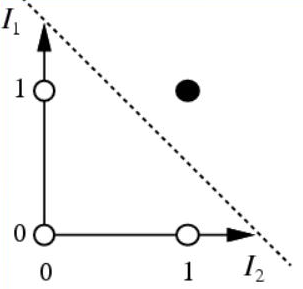
\includegraphics[width=\textwidth, height=\textwidth]{and.png}
                \caption{Puerta Lógica AND}
                \label{fig:and_logic_gate}
            \end{subfigure}
            \hfill
            \begin{subfigure}[H]{0.49\textwidth}
                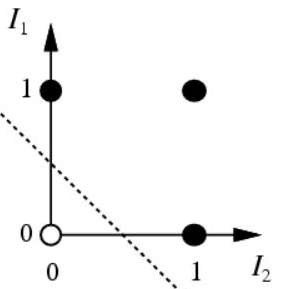
\includegraphics[width=\textwidth, height=\textwidth]{or.png}
                \caption{Puerta Lógica OR}
                \label{fig:or_logic_gate}
            \end{subfigure}
            \caption{Puertas Lógicas}
            \label{fig:logic_gates}
        \end{figure}

        \begin{figure}[H]
            \centering
            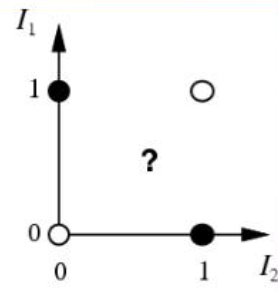
\includegraphics[width=5cm]{xor.png}
            \caption{Puerta Lógica XOR}
            \label{fig:xor_logic_gate}
        \end{figure}

        Además del uso de 2 o más capas dentro de la neurona, es indispensable el uso de una función de activación (Sección \ref{sec:activation}) que permite pasar la información de una neurona a otra dentro de un rango específico, lo cual se describirá en la siguiente sección.

        \subsubsection{Función de Activación} \label{sec:activation}

        Este método se utiliza cuando el modelo de RNA contiene dos o más neuronas, además proporciona al modelo una salida no lineal. Para este tipo de problemáticas donde tienen 3 entradas, se utiliza la siguiente fórmula: $f(w_1x_1 + w_2x_2 + w_3x_3 + b_0)$. Sin mencionar que las funciones de transferencia ayudan en cuestiones probabilísticas, ya que se representan en un rango de 0 a 1 \cite{renganathan2019}.

        Al hablar de funciones de activación, se deben comentar las más comunes:
        
        \begin{itemize}
            \item \textbf{Función Escalonada:} \\
                Esta función se utiliza para problemas de clasificación, ya que su salida es binaria, es decir, 0 o 1.
                \begin{figure}[H]
                    \centering
                    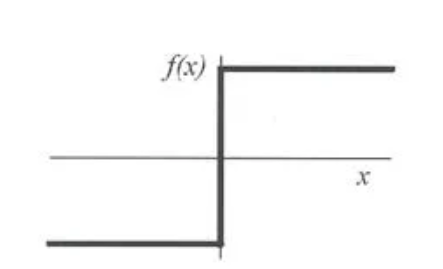
\includegraphics[width=5cm]{staggered.png}
                    \caption{Función Escalonada}
                    \label{fig:step_function}
                \end{figure}

                Dicha función está representada por:

                \[
                f(x) = \left\{ \begin{array}{lr} 
                0 & : x < 0 \\
                1 & : x \ge 0 
                \end{array} \right.
                \]
            
            \item \textbf{Función Sigmoide:} \\
                Esta función es una de las más comunes, ya que su salida es un rango de 0 a 1, lo que permite interpretarla como una probabilidad.
                \begin{figure}[H]
                    \centering
                    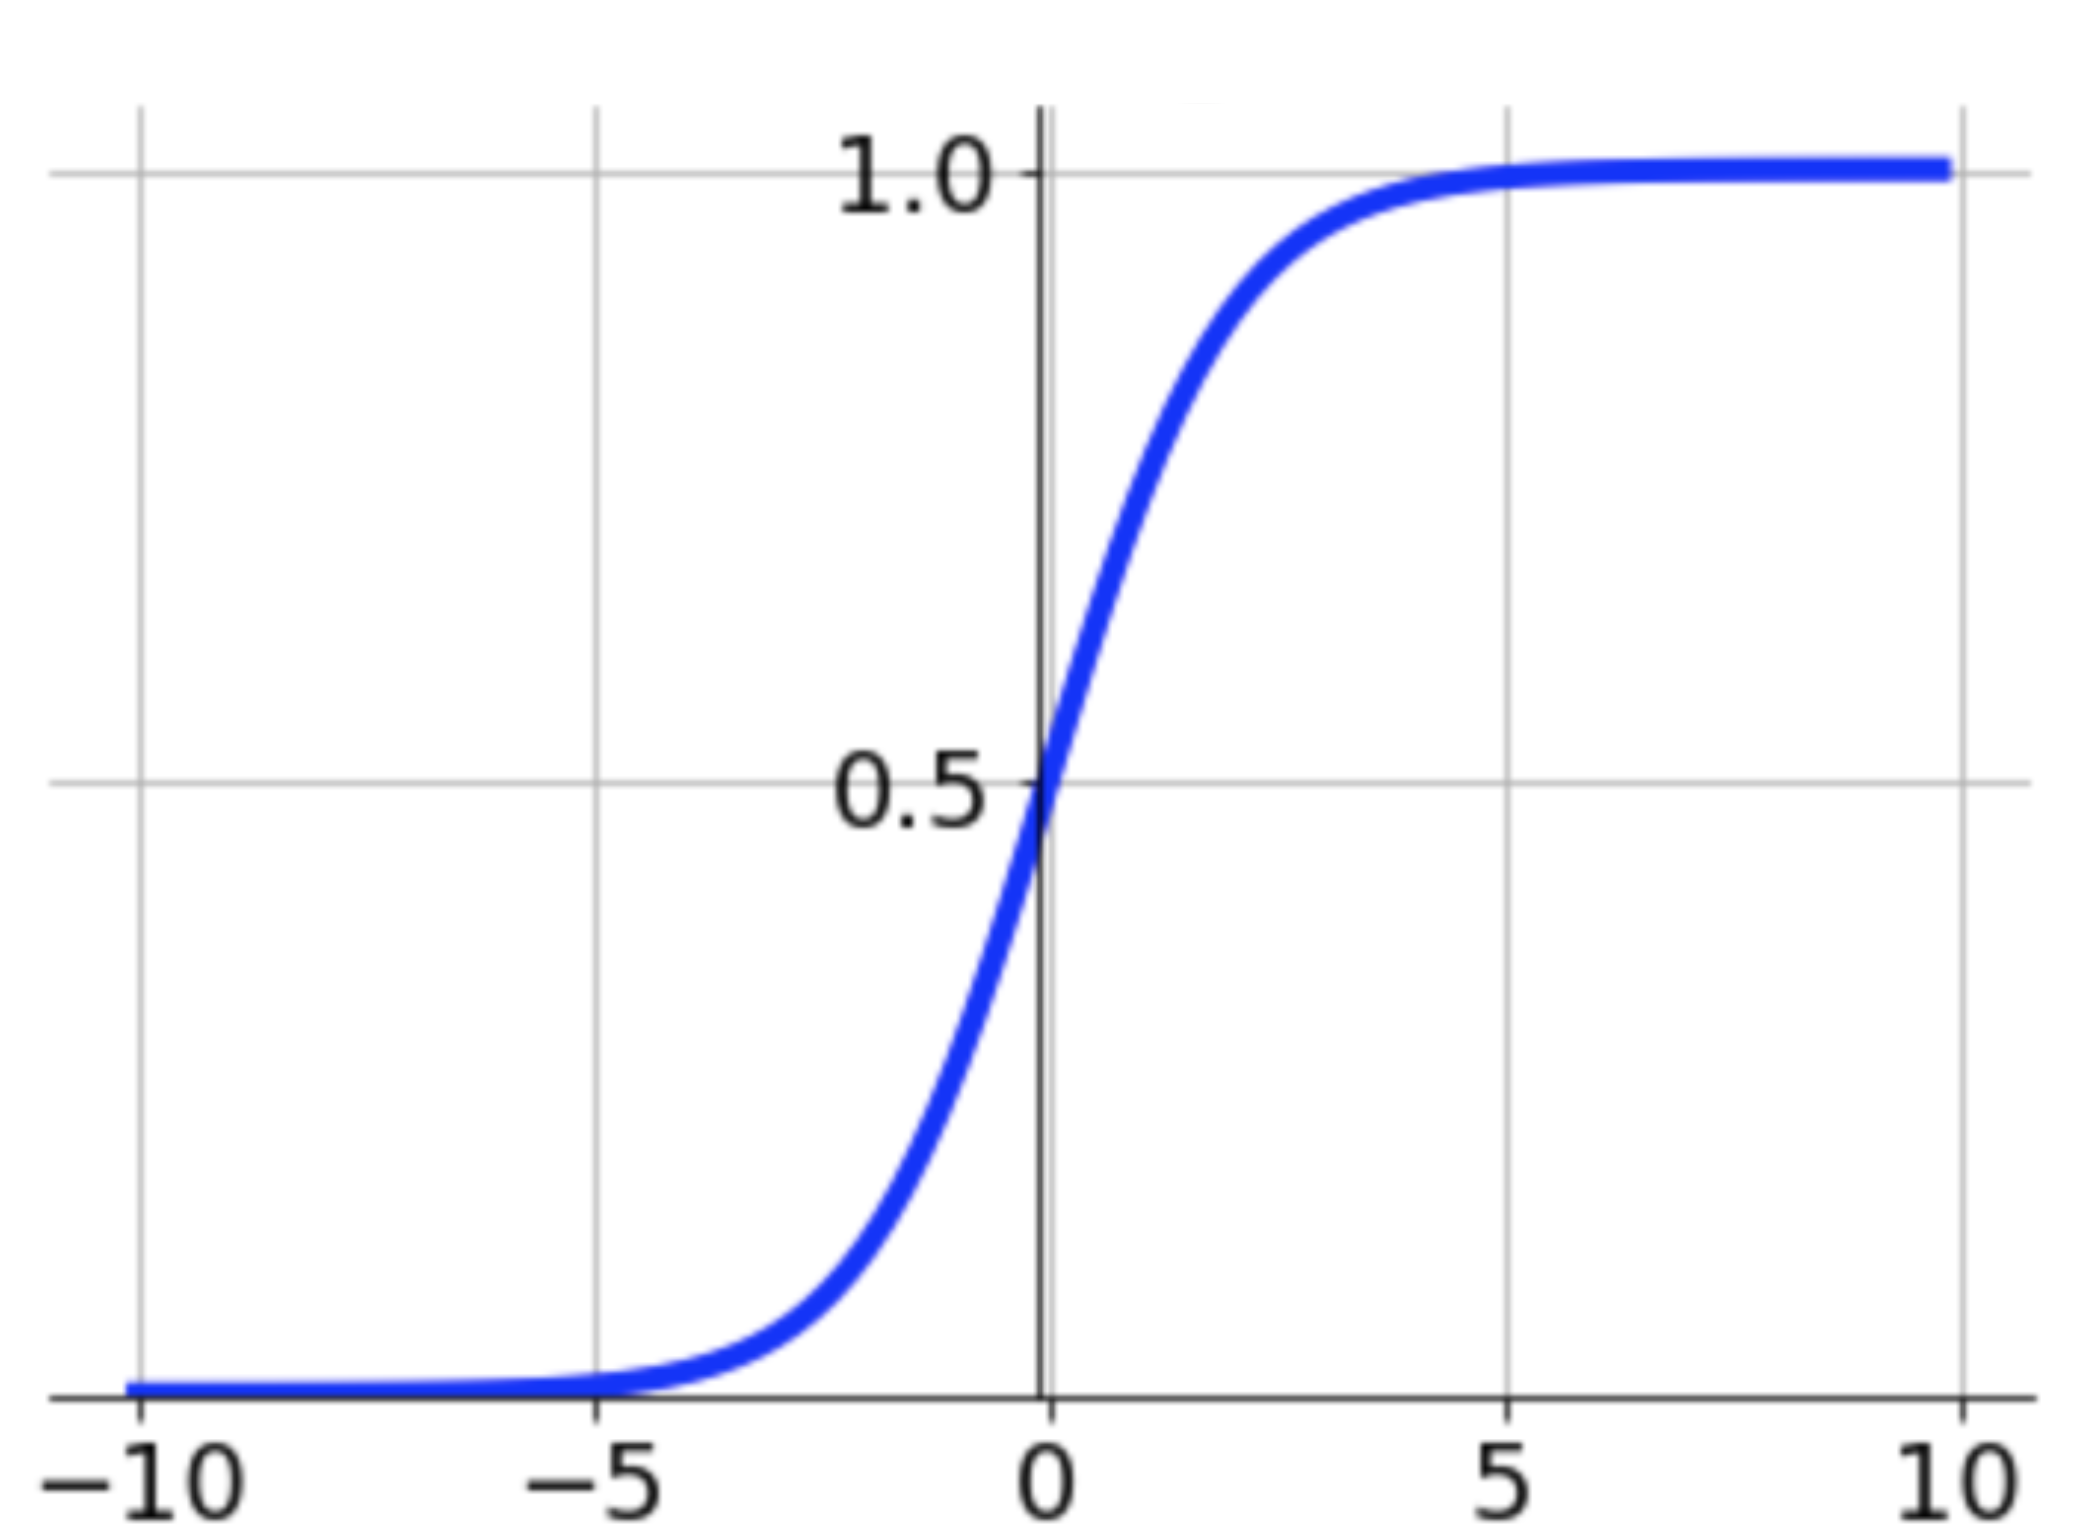
\includegraphics[width=5cm]{sigmoid.png}
                    \caption{Función Sigmoide}
                    \label{fig:sigmoid_function}
                \end{figure}

                Está representada por la siguiente fórmula:

                \[
                f(x) = \sigma(x) =  \frac{1}{1 + e^{-x}}
                \]

                Sin mencionar que este tipo de funciones es ajustable, lo cual es una característica importante del algoritmo de retropropagación (Sección: \ref{sec:backpropagation}).
            
            \item \textbf{Función de Unidad Rectificada Lineal (ReLU):} \\
                Esta función es la más utilizadas en RNAs ya que supera los problemas de desvanecimeinto del gradiente, además de ser más rápida en el entrenamiento. \\
                Es una función lineal que, cuando es positiva, toma el valor de la entrada, y cuando es negativa, toma el valor de 0.

                \begin{figure}[H]
                    \centering
                    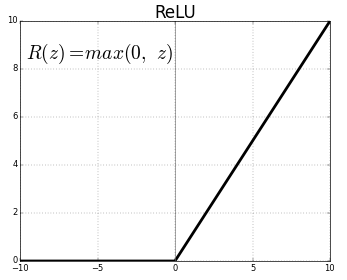
\includegraphics[width=6cm]{relu.png}
                    \caption{Función ReLU}
                    \label{fig:relu_function}
                \end{figure}

                Está representada por la siguiente fórmula:

                \[
                f(x) = \left\{ \begin{array}{lr} 
                0 & : x < 0 \\
                x & : x \ge 0 
                \end{array} \right.
                \]
            
            \item \textbf{Función Softmax:} \\
                Esta función se utiliza en la capa de salida de la red neuronal, ya que transforma las salidas en una representación probabilística, de tal manera que la suma de todas las probabilidades sea 1.
                \begin{figure}[H]
                    \centering
                    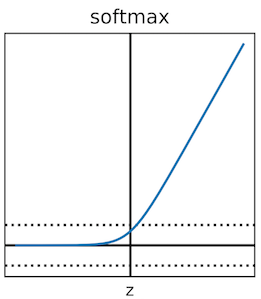
\includegraphics[width=6cm]{softmax.png}
                    \caption{Función Softmax}
                    \label{fig:softmax_function}
                \end{figure}

                Su representación matemática es:

                \[
                f(z)_j = \frac{e^{z_j}}{\sum_{K=1}^{K} e^{z_k}}
                \]
            
            \item \textbf{Función Tangente Hiperbólica:} \\
                Esta función es similar a la función sigmoide, pero su rango es de -1 a 1. También sufre de problemas de desvanecimiento del gradiente, lo que puede dificultar el entrenamiento de redes neuronales profundas.

                \begin{figure}[H]
                    \centering
                    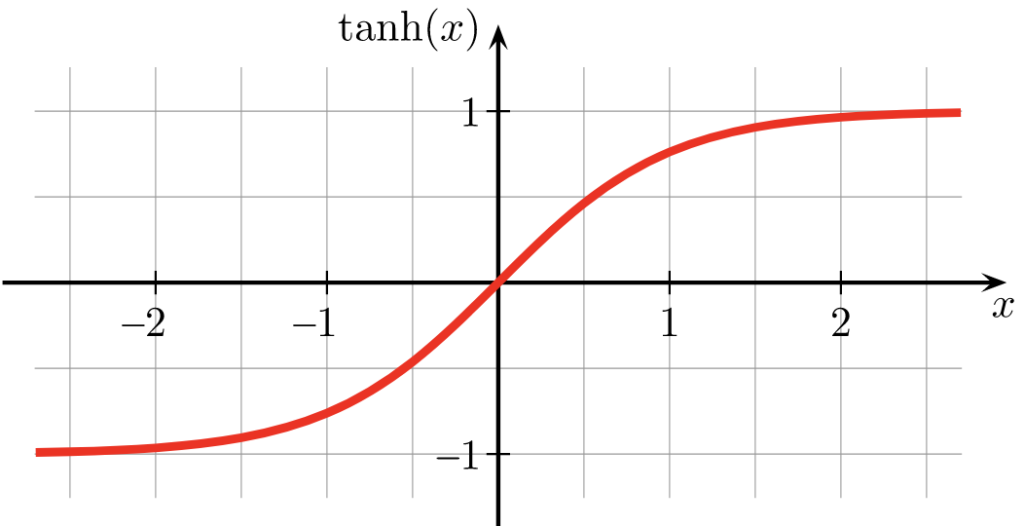
\includegraphics[width=6cm]{tanh.png}
                    \caption{Función Tangente Hiperbólica}
                    \label{fig:tanh_function}
                \end{figure}

                Su representación matemática es:

                \[
                f(x) = \tanh(x) = \frac{e^x - e^{-x}}{e^x + e^{-x}}
                \]
        
        \end{itemize}
        
        Las redes neuronales presentan diversas utilidades que ayudan a resolver problemas como no linealidad, mapeo entrada-salida, aprendizaje robusto a errores en los datos de entrenamiento, entre otros. Existen varios tipos de redes neuronales, como las redes neuronales de perceptrón multicapa y redes neuronales convolucionales, que se describirán brevemente más adelante.

    \subsection{Redes Neuronales de Perceptrón Multicapa}

        Las Redes Neuronales de Perceptrón Multicapa (MLP) pueden dividirse en dos capas (entrada y salida), pero también pueden tener tres o más capas (entrada, una o más capas ocultas y salida). En las capas ocultas, se pueden tener más de una fila de neuronas, que son las encargadas de realizar las operaciones para eliminar la linealidad de los datos. Como se comentó anteriormente en la sección \ref{sec:activation}, la linealidad de los datos se elimina con las funciones de activación, que modifican los parámetros de la red, permitiendo la elaboración de un plano tridimensional con el cual se puede encontrar la solución al problema planteado.

        Además, como se explicó anteriormente, no es recomendable trabajar con una sola neurona debido a los problemas al resolver tareas como XOR, donde se requieren dos líneas rectas para clasificar el problema correctamente.

        Como se puede observar en la Figura \ref{fig:multilayer_perceptron}, para este caso se cuenta con una MLP que consta de 4 capas: una de entrada, dos ocultas y una de salida. En las capas ocultas y de salida se lleva a cabo el procesamiento de las funciones de activación, mientras que en la capa de entrada no se aplica ninguna función de transferencia, ya que simplemente representa las entradas al modelo.

        \begin{figure}[H]
            \centering
            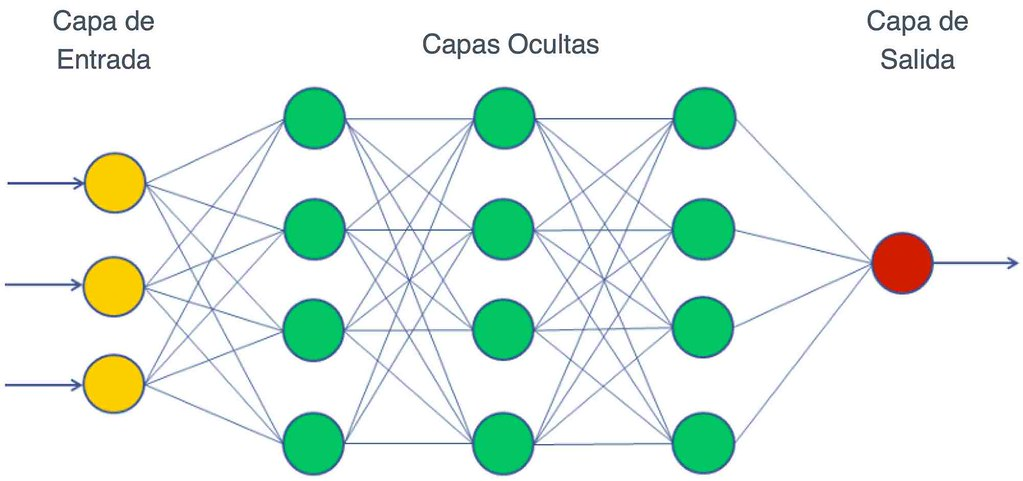
\includegraphics[width=\columnwidth]{multipercep.jpg}
            \caption{Red Neuronal Multicapa}
            \label{fig:multilayer_perceptron}
        \end{figure}

    \subsection{Algoritmo de Retropropagación} \label{sec:backpropagation}

        El algoritmo de retropropagación es un algoritmo de aprendizaje que permite que una red neuronal autoajuste todos sus parámetros para aprender una representación interna de la información que está procesando. Llegó para resolver la limitante del perceptrón, que solo resuelve problemas lineales, y se extiende a redes más complejas, es decir, a problemas no lineales.

        Mediante este algoritmo se obtienen las derivadas parciales del gradiente y los pesos, los cuales se utilizan para optimizar la red neuronal. También se deben calcular las derivadas del sesgo, que indican en qué capa se encuentra el error. El uso de estas derivadas parciales permite encontrar el error, y lo que realiza el algoritmo es retroceder hasta la neurona donde se encuentra el error, regresando desde la capa de salida hasta la capa de entrada.

        Para poder realizar todo este proceso de retropropagación, es necesario contar con una función de activación diferenciable.

    \subsection{Redes Neuronales Convolucionales}

        Las Redes Neuronales Convolucionales (CNN, por sus siglas en inglés) son redes profundas con una estructura especial. Están conformadas por tres tipos de capas: convolucionales, de agrupación y completamente conectadas.

        En las capas convolucionales, el filtro detecta características específicas dentro de la imagen de entrada, como bordes, colores, o texturas, y genera un mapa de características. En las capas de agrupación, se reduce la resolución espacial de la imagen, lo que permite reducir la cantidad de parámetros y el costo computacional. Finalmente, las capas completamente conectadas están encargadas de realizar la clasificación.

        Las CNN son muy útiles para el reconocimiento de imágenes, y se han utilizado en una amplia variedad de aplicaciones, desde la visión por computadora hasta la medicina y el reconocimiento de voz.


    \subsection{Aprendizaje Incremental}

        Con el paso del tiempo, la tecnología ha evolucionado, lo que ha llevado a un aumento en la cantidad de datos disponibles. El aprendizaje automático ha experimentado avances significativos, y los datos se generan y procesan con mayor frecuencia.

        Se puede definir una tarea de aprendizaje como incremental si los ejemplos de entrenamiento utilizados para resolverla se presentan de manera secuencial, generalmente uno a la vez. Si los resultados no son urgentes, este tipo de tareas puede ser resuelto mediante algoritmos de aprendizaje no incremental \cite{GiraudCarrier2000}. Un área donde el aprendizaje incremental es especialmente útil es en la \textit{robótica}, ya que estos sistemas requieren entrenamiento constante \cite{GiraudCarrier2000}.

        Este enfoque de aprendizaje fue inspirado por la forma en que los seres humanos aprenden y es más rápido, lo que llevó a su adopción en el campo del aprendizaje automático.

        Con el tiempo, el aprendizaje incremental se ha convertido en un paradigma del aprendizaje automático, donde el sistema toma nuevos ejemplos y los agrega a los ya aprendidos. A medida que el sistema aprende, los ejemplos previos pueden ser reemplazados por los nuevos \cite{liu2015}.

        \subsubsection{Algoritmos de Aprendizaje Incremental}

            Un algoritmo de aprendizaje incremental se define por los siguientes criterios:
            \begin{enumerate}
                \item Ser capaz de aprender y actualizarse con cada nuevo dato, etiquetado o no etiquetado.
                \item Conservar el conocimiento adquirido previamente.
                \item No requerir acceso a los datos originales.
                \item Ser capaz de generar nuevas clases o clusters cuando sea necesario, así como dividir o fusionar clusters según lo requiera el entorno.
                \item Tener una naturaleza dinámica, adaptándose a un entorno cambiante \cite{Deshmukh2013}.
            \end{enumerate}

            \begin{figure}[H]
                \centering
                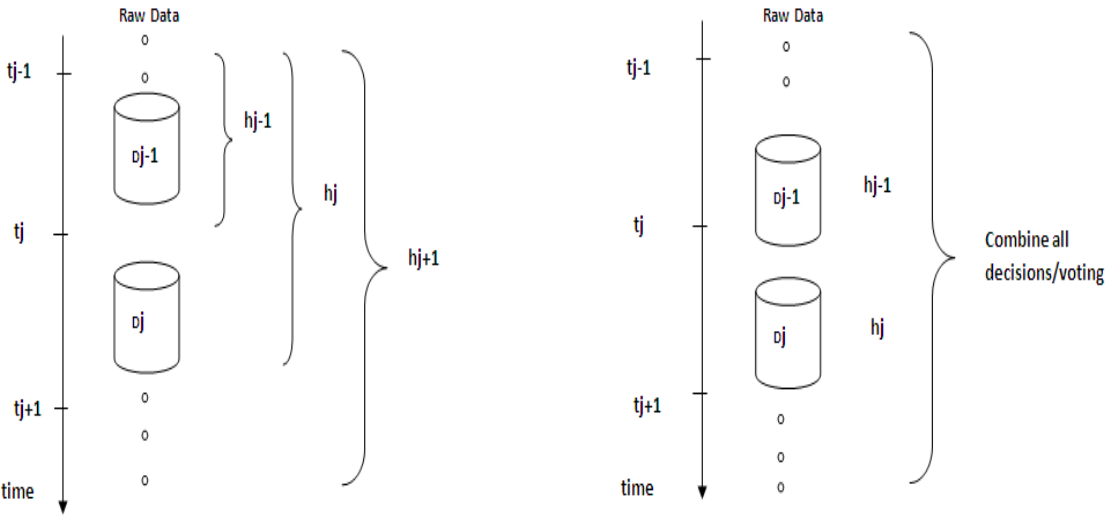
\includegraphics[width=\columnwidth]{MetodosAprendizajeIncremental.png}
                \caption{Dos enfoques tradicionales del aprendizaje incremental.}
                \label{fig:incremental_learning_algorithm}
            \end{figure}

            Como se observa en la Figura 11, el primer enfoque consiste en la acumulación de datos, donde, al recibir una nueva porción de datos \(D_j\), se descarta la hipótesis \(h_{j-1}\) y se genera una nueva hipótesis \(h_j\) basada en todos los datos disponibles hasta ese momento. En el segundo enfoque, al recibir una nueva porción de datos \(D_j\), se desarrolla una única hipótesis nueva o un conjunto de hipótesis nuevas basadas en los nuevos datos. Finalmente, se puede usar un mecanismo de votación para combinar todas las decisiones de las diferentes hipótesis y obtener la predicción final.

            El aprendizaje incremental tiene la ventaja de no requerir almacenamiento de los datos previos, ya que el conocimiento se guarda en las hipótesis generadas durante el proceso de aprendizaje.

            \begin{quote}
                \textit{``Un algoritmo de aprendizaje es incremental si, para cualquier muestra de entrenamiento dada:
                \begin{equation*}
                    e_1, e_2, ..., e_s
                \end{equation*}
                produce una secuencia de hipótesis
                \begin{equation*}
                    h_0, h_1, ..., h_n
                \end{equation*}
                tal que \(h_{i+1}\) depende solo de \(h_i\) y de la muestra actual \(e\)\cite{GiraudCarrier2000}.''}
            \end{quote}

            Como se observa, estos algoritmos permiten que la inteligencia artificial realice tareas de predicción de manera más eficiente.

            Un ejemplo de esta metodología es el proyecto \textit{COBWEB}, que categoriza el número de clusters y la pertenencia de dichos clusters utilizando una métrica probabilística global. Este proceso implica agregar nuevas categorías, actualizando las probabilidades con los nuevos datos recolectados \cite{fisher1987}.
    \section{Metodología}
    El primer paso a realizar en esta investigación es recrear el código mostrado en \cite{bullinaria2009}, donde se describe la implementación de una red  neuronal multicapa usando el algoritmo de entrenamiento backpropagation en el lenguaje de programación Python.  Para esto se utilizará el conjunto de datos de Optical Digits,  en donde se tendrá que preprocesar los datos, para eliminar registros inválidos. 

    Posteriormente se implementará una nueva versión del código en donde se experimentará con mas de dos capas de pesos duplicados para mejorar la tasa de olvido de información al momento de usar el aprendizaje incremental.  Para ello se explorará incrementando gradualmente el nueron de capas (esto no lo entendi,neuronas de capas?)de pesos duplicados, hasta llegar al punto en que mas capas no generen un decremento de las tasas de olvido/error.

(REVISEN LA REDACCIÓN Y MEJORENLA DE FAVOR)
    Cuando los dos proyectos se tengan, se realizar\'a una comparación, donde se ver\'a cual de estos dos experimentos
    es más eficaz en proyectos de la vida real.
    
\section{Cronograma de Actividades}
(EL CRONOGRAMA DE ACTIVIDADES DICE JOHN BULLINARIA EN LA PARTE DE ARRIBA, ELIMINAR ESO)

    \begin{figure}[H]
        \centering
        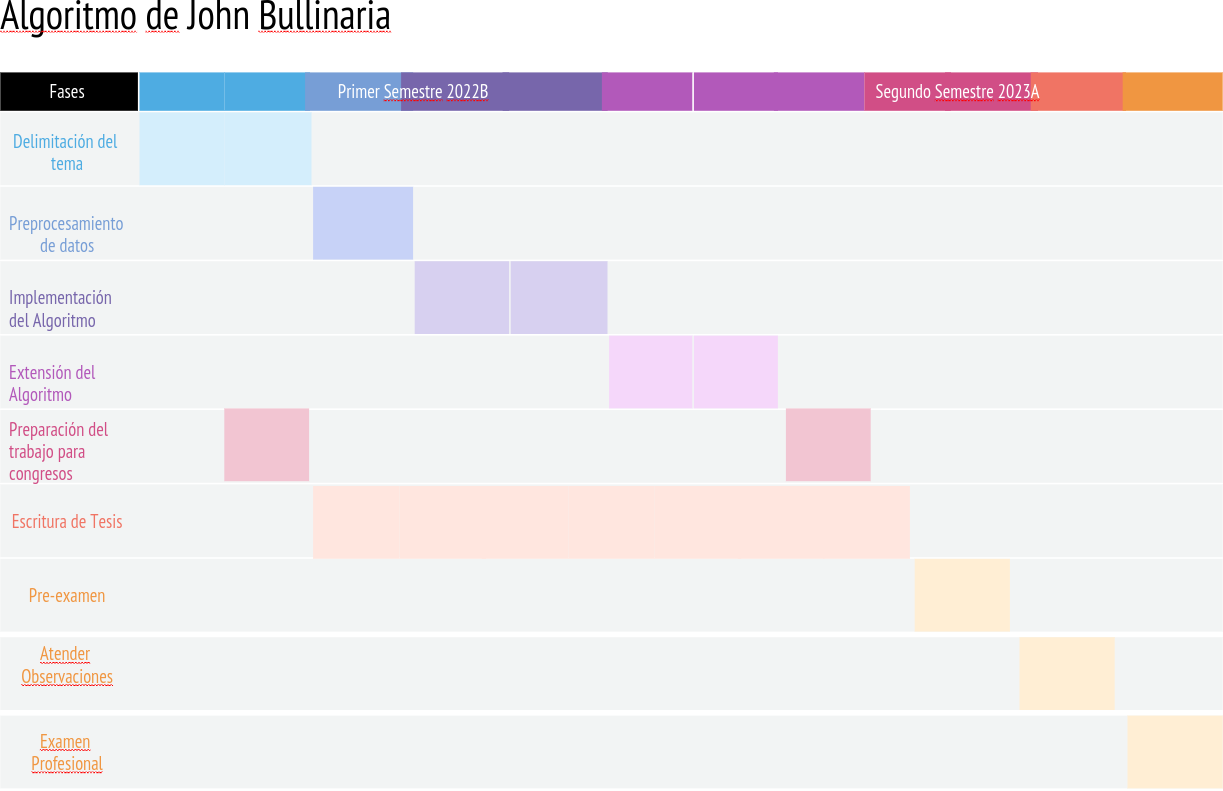
\includegraphics[width=\columnwidth]{diagramaGantt.png}
        %\caption{Elimine estoa horita, no hace falta ponerle un titulo, dado que es la únic figura en la sección}
        \label{fig:fig3}
    \end{figure}

\section{Organización del Capitulado}


	En el capitulo 2 se ver\'a lo que es el aprendizaje humano y el aprendizaje incremental con sus algoritmos, se describirán las redes neuronales artificiales.

En el capitulo 3 se implementar\'a el articulo de John A. Bullinaria, como funciona, resultado que da al pasar los datos que dice para comprobar que funciona como menciona en su art\'iculo. En el capitulo 4 se explicar\'a como se hará la modificación a su algoritmo, cuantas capas se van a poner, como se van a repartir las tazas de aprendizaje.

Posteriormente en el capitulo 5 se mostrar\'a una comparación de los resultados de ambos trabajos. En el capitulo 6 se verán las conclusiones y trabajo futuro.

    \ chapter{Organización del Capitulado}
 
 
	 En el capitulo 2 se explicar\'a lo que son y como funcionan las redes neuronales artificiales, as\i como la función de activación que es un método que utilizan estas0

	 Se describir\'an los tipos de redes neuronales, tanto de perceptron multicapa como convolucionales, y el algoritmo backpropagation.
	 Se mencionar\'a como es el aprendizaje en humanos, que este se divide en el aprendizaje activo y el aprendizaje con comprensión
	 Y para terminar se describirá el aprendizaje incremental y su algoritmo.\\
	 
	 En el capitulo 3 se implementar\'a el algoritmo de John A. Bullinaria, se verificar\'a su funcionamiento y los resultados que da al pasar los datos que dice para comprobar que es como menciona en su art\'iculo.\\
	 En el capitulo 4 se explicar\'a como se se extendió el algoritmo base permitiendo el uso de mas de dos pesos duplicados y se aplicaran los mismos datos de entrenamiento y de prueba que al algoritmo base.\\
	 
	 Posteriormente, en el capitulo 5 con los resultados obtenidos, se mostrar\'a una comparación de los resultados de ambos trabajos para notar si hubo una reducción significativa en las tasas de aprendizaje. En el capitulo 6 se verán las conclusiones y trabajo futuro.
    \section{Diagrama de Gantt}
\label{sec:gantt_chart}

  \begin{figure}[H]
    \centering
    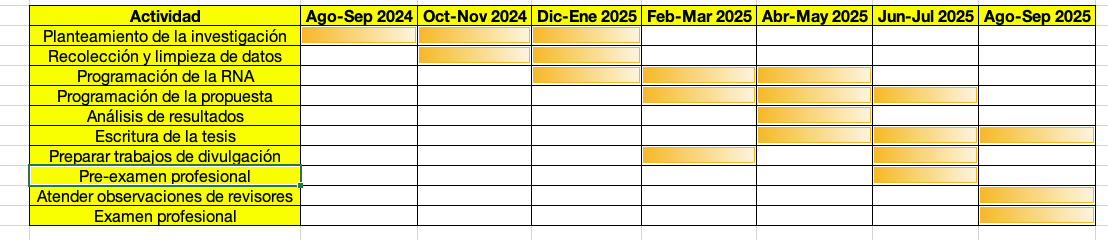
\includegraphics[width=1.0\textwidth]{gantt_chart/gantt_chart.png}
    \caption{Diagrama de Gantt}
    \label{fig:gantt_chart}
  \end{figure}
    
    %\printbibliography  
    %\bibliographystyle{acm}
    \bibliographystyle{plain}
    \bibliography{dataset}
    %\bibliography{BaseDatos2}

\end{document}